\section{Delay}
The delay in the system constitutes one of the main network effects in the system. In order to consider the delay on the system, the TrueTime simulation toolbox for MATLAB is utilized. 

In the simulation, a model for the delay needs to be found in order to implement it in TrueTime. The chosen approach is to model the delay as as the maximum possible delay appearing in the system. This has been obtained by adding the time required to make the information available in the microcontroller and the maximum time elapsed since the data is available until it is used by the microcontroller. 

The time required to make the data available can be divided into three. The time required to send the data, the transmission delay and the time it takes to decode the information in the microcontroller. The first and the third of these, can be found exactly as it is code execution time, the values obtained are 15 and 7.64 ms respectively. The transmission time can be found using the transmission speed of the Xbee modules. According to the datasheet \fxnote{source datasheet}, this is  115,2 kbit/s. With this speed and taking into account 21 bytes are transmitted, the transmission delay is 1.46 ms.

Once the information is on the microcontroller, the maximum time elapsed until the controller uses it is the sampling time minus the time needed to decode a package minus the execution time of the control loop. This is so because in the worst possible case, the package arrives just after the previous control loop finishes, then it is necessary to wait until the information is processed and until the next control loop is executed. 

\autoref{fig:delaycontrol} shows the different networked induced delays in the system and the maximum delay. 
\begin{figure}[H]
	\centering
	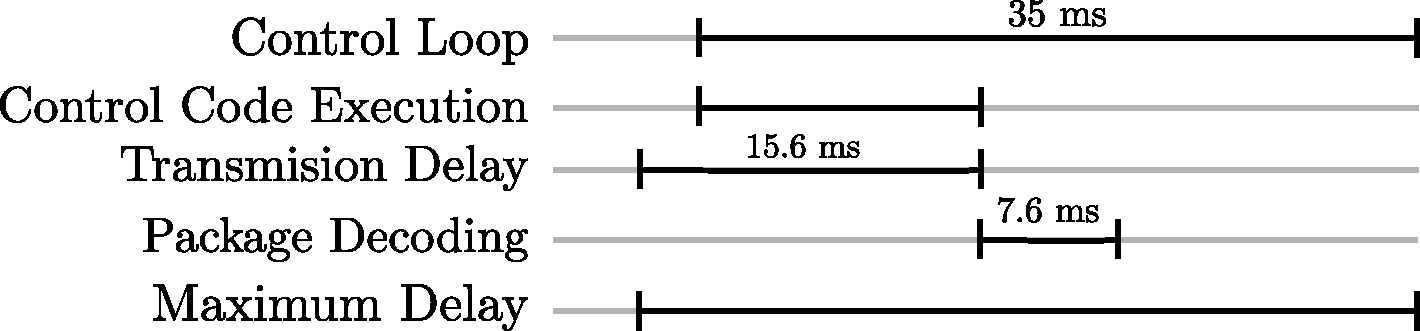
\includegraphics[width=.6\textwidth]{figures/maxDelay.pdf}
	\caption{Delays in the packages transmitted to the microcontroller and maximum delay.\fxnote{Check times}}
	\label{fig:delaycontrol}
\end{figure}

After all considerations, the value of the delay used in the simulation is 50.6 ms\fxnote{Check delay}.

%since the information is obtained until it is sent through the network, the transmission delay and the time needed to process the information in the microcontroller. being exponentially distributed. \autoref{eq:exponentialdist} shows the probability and cumulative density functions of the exponential distribution.
%\begin{flalign}
%		f=-\lambda\mathrm{e}^{-\lambda t}\mathrm{;}\ \ \ \ \  F=1-\mathrm{e}^{-\lambda t}
%		\label{eq:exponentialdist}
%\end{flalign}
%\begin{where}
%	\va{f} {is the probability density function} { }
%	\va{F} {is the cumulative density function} { }
%	\va{\lambda} {is the rate parameter} { }
%	\va{t} {is time} { }
%\end{where}
%The parameter lambda can be interpreted as the inverse of the mean time between observations, that is, the mean delay in the system. The value for this parameter has been found experimentally by measuring and averaging the experienced delays in \fxnote{PUT NUMBER} transmissions. The detailed experiments can be seen in \fxnote{APPENDIX WITH DATA}. The average delay obtained is \fxnote{PUT NUMBER} which leads to a value for $\lambda$ of \fxnote{PUT NUMBER}
 
%To generate the exponential distributed delays, the inverse transformation theorem has been applied. This theorem allows to transform an uniformly distributed random variable, easier to generate, into a random variable distributed with any other known cumulative density function. \autoref{eq:invtransthorem} illustrates this theorem.
%\begin{flalign}
%	\mathrm{Y}= F^{-1}\mathrm{X}
%	\label{eq:invtransthorem}
%\end{flalign}
%\begin{where}
%	\va{F} {is the desired cumulative density function for the random variable} { }
%	\va{\mathrm{X}} {is a uniformly distributed random variable} {}
%	\va{\mathrm{Y}} {is a random variable distributed according to the cumulative density function $F$} {}
%\end{where}

%The final expression obtained can be seen in \autoref{eq:formuladelay}.
%\begin{flalign}
%	\mathrm{delay}= -\frac{\ln(1-\mathrm{X})}{\lambda}
%	\label{eq:formuladelay}
%\end{flalign}






